\documentclass[12pt]{article}
\usepackage{lineno}
\usepackage[spanish]{babel}
\usepackage{amsmath}
\usepackage{graphicx}
\usepackage[utf8]{inputenc}
\usepackage{pslatex}
\usepackage{theorem}
\usepackage{color}
\newtheorem{teorema}{Teorema}
\newtheorem{proposicion}{Proposición}
\newtheorem{nota}{Nota}
\DeclareGraphicsExtensions{.pdf,.png,.jpg}


\title{Estrategias de determinante cero de W.H. Press y F.J. Dyson}
\date{}
\author{Exequiel Aguirre}
% document start
\begin{document}
%\linenumbers
\maketitle

\begin{abstract}
El juego del dilema del prisionero, en su versión de dos jugadores, puede ser usado como modelo para 
muchas situaciones del mundo real, que involucran cooperativismo y competencia. Se asume en general, que no hay 
una estrategia donde, unilateralmente, se pueda forzar a recibir una recompensa injusta.\newline
En el artículo publicado por W.H. Press y F.J. Dyson, se muestra que existen estrategias con esa característica.
Con dichas estrategias, un jugador puede forzar el puntaje del oponente o establecer una relación lineal entre
el puntaje propio y el del oponente.\newline
En este trabajo, se pretende explicar lo expuesto en el paper original de W.H. Press y F.J. Dyson, completando
algunos cálculos y aplicarlos en una simulación.
\end{abstract}




\section{Introducción}
El dilema del prisionero provee un  marco para entender como dar con un balance entre cooperación y competencia, y es
por eso una herramienta muy útil para tomar deciciones estratégicas.
Tiene aplicaciones en diversas áreas, como por ejemplo: economía,política,biología,psicología y sociología.\newline
El juego se puede presentar de la siguiente manera:\newline
Dos miembros de una banda criminal son capturados por la policia e interrogados, por separado.
Cada criminal tiene dos opciones, cooperar con su compañero o no cooperar.
De ahora en adelante nos referiremos a cada criminal como, jugador X y jugador Y.
Si X e Y cooperan, ambos ganan una recompensa R, si uno de ellos no coopera recibe un pago mayor T, mientras que el
jugador que coopera recibe una recompensa menor, S, usualmente cero. Si ambos no cooperan, entonces reciben una recompensa P.
Para que el juego sea de interés, se debe satisfacer que $T >  R > P > S$ y $2R > T+S$.
Los valores usuales son (T,R,P,S)=(5,3,1,0)
\begin{center}
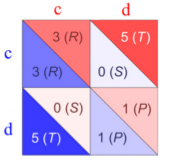
\includegraphics[height=3cm]{./pd.png}
\end{center}


El dilema del prisionero iterado, consiste en sucesivas partidas jugadas por, digamos X e Y.
Aquí los jugadores podrían basar sus jugadas en las jugadas anteriores.Sería natural pensar que el jugador que es
capaz de recordar más jugadas, podría confeccionar una estrategia más eficiente y así llevar ventaja.
Se va a probar luego, que esto no es así, y que solo importa la última jugada. Es por eso que las estrategias seran elaboradas
a partir de el último resultado, sin pérdida de generalidad.
Es decir, cada jugador va a basar su estrategia en el resultado xy $\in$ (cc,cd,dc,dd) donde c significa cooperar y d, no cooperar 
(defect en inglés). La estrategia de X, p=($p_1,p_2,p_3,p_4$) son las probabilidades de cooperar en cada una de las situaciones 
anteriores. En forma análoga, la estrategia de Y es q=($q_1,q_2,q_3,q_4$) visto desde su perspectiva yx $\in$ (cc,cd,dc,dd).

\section{Resultados}
\subsection{Estrategias de determinante cero}
Si bien es posible realizar una simulación del juego movimiento por movimiento uno podría evitar esto con una matriz
de transición de Markov. Esta matriz es generada a partir de las estrategias p y q.
$$M=
\begin{bmatrix}
 p_1 q_1 &p_1(1-q_1) &(1-p_1)q_1 &(1-p_1)(1-q_1)\\
 p_2 q_3 &p_2(1-q_3) &(1-p_2)q_3 &(1-p_2)(1-q_3)\\
 p_3 q_2 &p_3(1-q_2) &(1-p_3)q_2 &(1-p_3)(1-q_2)\\
 p_4 q_4 &p_4(1-q_4) &(1-p_4)q_4 &(1-p_4)(1-q_4)\\
\end{bmatrix}
$$
El valor $M_{ij}$ representa la probabilidad de pasar de un estado i a un estado j donde, i,j estan asociados a una 
estrategia en (cc,cd,dc,dd), según la perspectiva de cada jugador.
Por ejemplo, $M_{32}$ representa la probabilidad de pasar de un estado dc a cd.\newline
Definición: Un vector $v_s$ tal que,
\begin{center}
$v_s^T M = v_s^T$
\end{center}
y sus componentes suman 1, es llamado  vector estacionario.\newline
Notar que cualquier vector $v$ proporcional a $v_s$ también cumple con la condición:
\begin{center}
$v^T M = v^T$
\end{center}
Es decir, un autovector (a izquierda) asociado al autovalor 1.
Con $v$ y el vector de pagos asociado a cada jugador, uno puede calcular el resultado del juego.

Dado que M tiene un autovector asociado al autovalor 1, la matriz $M'$:=M-I es singular y por ende, de 
determinante cero.\newline
De álgebra lineal se tiene el siguiente resultado:\newline
\begin{center}
$Adj(M')M' = det(M')I=0$
\end{center}
Donde Adj($M'$) es la matriz Adjunta de $M'$\footnote{Para más información sobre este resultado y las definiciones involucradas ver \cite{Ho}.}.\newline 
Sea A:=Adj($M'$), entonces por la igualdad anterior, tenemos que:
\begin{center}
$AM'=A(M-I)=0 \Rightarrow AM=A$
\end{center}
Es decir, que el elemento 
\begin{center}
$(AM)_{ij}=\sum_{k=1}^4 A_{ik} M_{kj} = A_{ij}$
\end{center}
Ahora, sea w la n-esima fila de A.
\begin{center}
$w:=(w_1,w_2,w_3,w_4)=(A_{n1},A_{n2},A_{n3},A_{n4})$
\end{center}
Entonces, el j-esimo elemento del vector (w M) es,
\begin{center}
$(w M)_j=\sum_{k=1}^4 w_k M_{kj} =\sum_{k=1}^4 A_{nk} M_{kj} = A_{nj}=w_j$
\end{center}
Es decir que w M= w, por ende, w es proporcional a v.
Dado que n es arbitrario, se puede concluir que cada fila de Adj($M'$) es proporcional a v.
\footnote{Esta afirmación no es trivial, proviene de aplicar el teorema de Perron-Frobenius. Para más información ver \cite{Ha}.}

Sea w, la cuarta fila de la matriz A, 
\begin{center}
$w:=(w_1,w_2,w_3,w_4)=(A_{41},A_{42},A_{43},A_{44})$.
\end{center}
Nos enfocaremos en la primera componente de w, por un momento.
\begin{center}
 $$
 w_1=A_{41}=Adj(M')_{41}=(-1)^{4+1} C_{14}=- det
 \begin{bmatrix}
 p_2 q_3 & p_2(1-q_3)-1 &(1-p_2)q_3 \\
 p_3 q_2 & p_3(1-q_2) &(1-p_3)q_2 -1 \\ 
 p_4 q_4 & p_4(1-q_4) &(1-p_4)q_4 \\ 
 \end{bmatrix}
 $$
 \end{center}
 Donde $(-1)^{4+1} C_{14}$ es el cofactor de $M'_{41}$. Este determinante no se modifica si sumamos la 
 primera columna de $M'$ a la segunda y tercera, obteniendo
 \begin{center}
 $$w_1=- det
 \begin{bmatrix}
 p_2q_3 & p_2(1-q_3)-1+p_2q_3 &(1-p_2)q_3+p_2q_3 \\
 p_3q_2 & p_3(1-q_2)+p_3q_2 &(1-p_3)q_2 -1+p_3q_2 \\ 
 p_4q_4 & p_4(1-q_4)+p_4q_4 &(1-p_4)q_4+p_4q_4 \\ 
 \end{bmatrix}
 =- det
 \begin{bmatrix}
 p_2q_3 & p_2-1 & q_3 \\
 p_3q_2 & p_3 & q_2-1 \\ 
 p_4q_4 & p_4 & q_4 \\ 
 \end{bmatrix} 
 $$
\end{center} 
Llamemos $W_1$ a esta última matriz.Un cálculo similar se puede realizar y obtener matrices $W_2,W_3,W_4$ 
correspondientes a $w_2,w_3,w_4$ respectivamente. Es decir que las componentes de v, son salvo un signo y una constante c, 
determinantes de una matriz de este tipo.
Ahora sea, $f=(f_1,f_2,f_3,f_4)$,entonces,
\begin{center}
$$
D(p,q,f):=det
\begin{bmatrix}
 p_1q_1-1 & p_1-1 & q_1-1 & f_1 \\
 p_2q_3 & p_2-1 & q_3 & f_2\\
 p_3q_2 & p_3 & q_2-1  & f_3\\ 
 p_4q_4 & p_4 & q_4 & f_4\\ 
 \end{bmatrix} 
 $$
 $$
 =-det(W_1)f_1 +det(W_2)f_2 -det(W_3)f_3 +det(W_4)f_4 
 = c v \cdot f
 $$
\end{center}
Notar que la segunda columna $\tilde{p}= (p_1-1,p_2-1,p_3,p_4)$ está solo bajo el control de X.
Analogamente la tercera columna $\tilde{q}=(q_1-1,q_3,q_2-1,q_4)$ esta bajo el control de Y.\newline
Sean $S_X:=(R,S,T,P)$ , $S_Y:=(R,T,S,P)$ los vectores de pago de X e Y respectivamente.
En su estado estacionario, podemos escribir los respectivos puntajes finales, como:
\begin{center}
$s_X=\frac{v \cdot S_X}{v \cdot \overline1} = \frac{D(p,q,S_X)}{D(p,q,\overline1)}$ , 
$s_Y=\frac{v \cdot S_Y}{v \cdot \overline1} = \frac{D(p,q,S_Y)}{D(p,q,\overline1)}$
\end{center}
Donde el vector $\overline1:=(1,1,1,1)$.Estos denominadores son necesarios para que las
componentes sumen 1, (requerido en un para un vector de probabilidad estacionario).
Dado que los puntajes s, dependen linealmente de los vectores de pago S, lo mismo
sucede para una combinación lineal de los mismos.
\begin{center}
 $\alpha s_X + \beta s_Y + \gamma=\frac{D(p,q,\alpha S_X + \beta S_Y + \gamma\cdot \overline1)}{D(p,q,\overline1)}$
\end{center}
Esta es de alguna manera la ecuación más importante, pues tanto X como Y pueden elegir una
estrategia que anule el numerador. Es decir, si X elije una estrategia 
$\tilde{p}= \alpha S_X + \beta S_Y + \gamma\cdot \overline1$, o si Y elije una estrategia
$\tilde{q}= \alpha S_X + \beta S_Y + \gamma\cdot \overline1$ entonces 

\begin{center}
$\alpha s_X + \beta s_Y + \gamma$=0
\end{center}
Estas son las llamadas, estrategias de determinante cero.

\subsection{X define unilateralmente el puntaje de Y}
Un caso particular de una estrategia de determinante cero, es donde X define el puntaje de Y.
Eligiendo $\alpha=0$ en la ecuación anterior, obtenemos: $\tilde{p}=\beta S_Y + \gamma \overline1$
Esto nos define cuatro ecuaciones:
$$p_1-1=\beta R + \gamma$$
$$p_2-1=\beta T + \gamma$$
$$p_3=\beta S + \gamma$$
$$p_4=\beta P + \gamma$$
Eliminando $\beta$ y $\gamma$, obtenemos,
$$p_2=\frac{p_1(T-P)-(1-p_4)(T-R)}{R-P}$$
$$p_3=\frac{(1-p_1)(P-S)+p_4(R-S)}{R-P}$$
$$s_Y=\frac{-\gamma}{\beta}=\frac{\beta R+ 1-p_1}{\beta}=\frac{(1-p_1)P+p_4 R}{p_4-p_1+1}$$
De esta última ecuación, se desprende que X puede forzar el puntaje de Y,
$$P\leq s_Y\leq R $$

\subsection{X intenta definir su propio puntaje}
Analogamente al caso anterior,con $\tilde{p}=\alpha S_X + \gamma\overline1$  obtenemos,
$$p_2=\frac{(1+p_4)(R-S)-p_1(P-S)}{R-P}\geq 1$$
$$p_3=\frac{-(1-p_1)(T-P)-p_4(T-R)}{R-P}\leq 0$$
Estas ecuaciones nos indican que la única estrategia posible es p=(1,1,0,0), es decir
X no puede decidir su puntaje unilateralmente.


\subsection{X demanda y obtiene una porción del puntaje de Y}
El jugador X, ahora pretende establecer una relación lineal entre su puntaje y el de Y,
$$(s_X -P)=\chi (s_y-P)$$
con $\chi \geq 1$ (para así beneficiarse). Equivalentemente,
$$(s_X -P)-\chi (s_y-P)=0 \Leftrightarrow \phi[(s_X -P)-\chi (s_y-P)]=0 \Leftrightarrow \frac{\phi}{P-S}[(s_X -P)-\chi (s_y-P)]=0$$
Con $\phi>0$. X puede forzar esta relación eligiendo la estrategia
$$\tilde{p}=\frac{\phi}{P-S}[(S_X-P\cdot\overline1)\ - \chi (S_Y-P\cdot\overline1)]$$
Así obtenemos,
$$p_1=1-\frac{\phi}{P-S}(R-P)(\chi-1)$$
$$p_2=1-\phi(1+\chi \frac{T-P}{P-S})$$
$$p_3=\phi(\frac{T-P}{P-S}+\chi )$$
$$p_4=0$$
De la ecuación de $p_2$ se puede verificar que,
$$\phi(1+\chi\frac{T-P}{P-S})\leq 1 \Rightarrow \phi\leq(1+\chi \frac{T-P}{P-S})^{-1}=\frac{P-S}{(P-S) + \chi(T-P)}$$
Ahora el puntaje de X depende del puntaje de Y.Ambos son máximos cuando Y coopera plenamente, con
q=(1,1,1,1). En este caso, el puntaje de X es,
$$s_X= \frac{D(p,q,S_X)}{D(p,q,\overline1)}=\frac{(\chi R + (1-\chi)P)T-\chi RS+(\chi-1)PR}{T-\chi S+(\chi-1)R}=$$
$$\frac{P(T-R)+\chi[R(T-S)-P(T-R)]}{(T-R)+\chi(R-S)}$$
Esta situación se puede hacer más concreta, con los valores convencionales (T,R,P,S)=(5,3,1,0), entonces,
$$p=[1-2\phi(\chi-1),1-\phi(4 \chi+1),\phi(\chi+4),0]$$
Donde los mejores puntajes posibles para X e Y son,
$$s_X=\frac{2+13\chi}{2+3\chi}, s_Y=\frac{12+3\chi}{2+3\chi}$$
El parametro $\chi$ es conocido como el factor de extorsión. En el caso particular donde, $\chi=1$ , y $\phi =1/5$
entonces la estrategia p=(1,0,1,0) es la estrategia de tit-for-tat.



\subsection{Resultados numéricos}
A continuación se presenta una serie de resultados obtenidos a partir de un programa que simula múltiples jugadas, de dos
jugadores, X e Y. La estrategia de X será una estrategia de determinante cero, mientras que la estrategia de Y será 
generada aleatoriamente, al empezar el juego.
En las siguientes tablas se mostrarán los resultados de las distintas estrategias y sus variantes, donde N es la cantidad de
jugadas y $\overline s_Y$ es el promedio del puntaje del jugador Y. Los valores de (R,T,P,S) son los usuales.\newpage

X fuerza el puntaje de Y, $s_Y=1$
\begin{center}
  \begin{tabular}{| l | l |}
    \hline
    N & $\overline s_Y$ \\\hline
    100 & 1.18 \\\hline
    1000 & 0.985 \\\hline
    10000 & 0.9861 \\\hline
    100000 & 0.99283 \\\hline
    1000000 & 1.001047 \\\hline
    10000000 & 0.9994806 \\\hline
    
  \end{tabular}
\end{center}
Estrategia extorsiva con $\chi=1$ (X fuerza un empate)
\begin{center}
  \begin{tabular}{| l | l | l |}    
    \hline
    N & $\overline s_X$ & $\overline s_Y$ \\\hline
    100 & 2.04 & 2.09 \\\hline
    1000 & 2.492 & 2.497 \\\hline
    10000 & 2.1624 & 2.1629 \\\hline
    100000 & 1.95382 & 1.95382 \\\hline
  \end{tabular}
\end{center}
Estrategia extorsiva con $\chi=2$. 
\begin{center}
  \begin{tabular}{| l | l | l | l |}
    \hline
    N & $\overline s_X$ & $\overline
    s_Y$ & $\overline s_Y$ esperado ($s_Y=\frac{(s_X-P)}{\chi} + P$)\\\hline
    100 & 2.52 & 1.62 & 1.76\\\hline
    1000 & 2.683 & 1.848 & 1.8415  \\\hline
    10000 & 2.7489 & 1.8974 & 1.8744\\\hline
    100000 & 2.4403 & 1.7238 & 1.7202 \\\hline
    1000000 & 2.429798 & 1.716298 & 1.7149 \\\hline
  \end{tabular}
\end{center}

Se concluye con un ejemplo de aplicación de las estrategias de determinante cero.
Supongamos que las ganacias de Coca-cola y PepsiCo se dan de la siguiente manera:
\begin{enumerate}
 \item Si ambas mantienen precios altos, las ganancias de cada compañia se incrementan
 en \$ 500 millones. 
 \item Si uno deja caer el precio,(no coopera) pero el otro mantiene (coopera) entonces 
 el primero verá un incremento de \$750 millones, mientras que el segundo no verá una modificación en sus ganancias.
 \item Si ambas dejan caer el precio,entonces ambos verán un incremento de \$250 millones.
\end{enumerate}
 
La matriz de pagos se ve de la siguiente forma:

\begin{tabular}{|l|r| l|}
  \hline   
     & c & d \\\hline
   c & 500,500 & 0,750 \\ \hline
   d & 750,0 & 250,250 \\  \hline  
\end{tabular} 

Si una de estas empresas decidiera utilizar una estrategia extorsiva, el resultado podría ser el
siguiente:

Estrategia extorsiva con $\chi=2$. 
\begin{center}
  \begin{tabular}{| l | l | l |}
    \hline
    N & $\overline s_X$ & $\overline s_Y$ \\\hline
    10 & 350.0 &350.0 \\\hline
    100 & 412.5 & 345.0 \\\hline
    1000 & 466.0 & 353.5 \\\hline
    10000 & 508.575 & 378.225 \\\hline    
  \end{tabular}
\end{center}


\subsection{Apéndice: El jugador con menos memoria,fija las reglas de juego}
Como se mencionaba al principio de este trabajo, se podría pensar que aquel jugador
con una estrategia basada en múltiples jugadas anteriores está en ventaja respecto de
un jugador con estrategias elaboradas basadas en una menor cantidad de jugadas.
Ese no es el caso, cuando bajo iguales condiciones, el juego es repetido  indefinidamente.
Por iguales condiciones, se quiere decir, mismos movimientos permitidos y mismos vectores
de pago.\newline
Sean X e Y variables aleatorias con valores x,y correspondientes a los moviemientos en una iteración dada.
Dado que los puntajes solo dependen de (x,y) en cada jugada, es suficiente con examinar la esperanza
de la probabilidad conjunta de  (X,Y) sobre la historia H.
Sea $H=[H_0,H_1]$ donde $H_0$ es la historia reciente compartida por X e Y, y $H_1$ es la historia con más antiguedad
solo vista por Y. Entonces,
$$<P(x,y|H_0,H_1)>_{H_0,H_1}=\sum_{H_0,H_1}P(x,y|H_0,H_1) P(H_0,H_1)=$$
$$\sum_{H_0,H_1} P(x|H_0)P(y|H_0,H_1)P(H_0,H_1)=\sum_{H_0} P(x|H_0) \sum_{H_1} P(y|H_0,H_1)P(H_0,H_1)=$$
$$\sum_{H_0}P(x|H_0)\sum_{H_1}P(y|H_0,H_1)P(H_0)P(H_1|H_0) =\sum_{H_0}P(x|H_0)P(H_0) \sum_{H_1}P(y|H_0,H_1)P(H_1|H_0)=^*$$
$$\sum_{H_0}P(x|H_0)P(H_0)\sum_{H_1} P(y,H_1|H_0)=\sum_{H_0}P(x|H_0)P(H_0)P(y|H_0)=$$
$$\sum_{H_0}P(x,y|H_0)P(H_0)=<P(x,y|H_0)>_{H_0} $$

La primera igualdad es la definición de esperanza, la segunda igualdad proviene del hecho que x e y son independientes.La 
igualdad *,proviene de,
$$P(y|H_0,H_1)P(H_1|H_0)=\frac{P(y,H_0,H_1)}{P(H_0,H_1)} \frac{P(H_1,H_0)}{P(H_0)}=\frac{P(y,H_1,H_0)}{P(H_0)}=P(y,H_1|H_0)$$
Lo notable es que el juego es determinado solo por $H_0$ donde Y juega la estrategia,
$$P(y|H_0)=\sum_{H_1}P(y,H_1|H_0)$$
Dado que esta estrategia solo depende de $H_0$, es una estrategia de corta memoria que produce el mismo
resultado que la estrategia original.


\newpage
 \section{}
  \begin{thebibliography}{1}
  \bibitem{Ha} Hauert Ch, Schuster HG (1997) Effects of increasing the number of players and memory steps in the Iterated Prisoner’s Dilemma, a numerical approach. Proc Biol Sci 264:513–519.
  \bibitem{Ho}  Hoffman K.,Kunze R.  \emph{``Linear Algebra''},Prentice-Hall, 1973 (155-161)
  \bibitem{PI}  Picardo E. {\em (2013) Utilizing Prisoner’s Dilemma In Business And The Economy }
  \bibitem{PR}  Press W. H. , Dyson F. J.  {\em (2012) Iterated Prisioner's Dilema contains strategies that dominate any evolutionary opponent}  
  \end{thebibliography}


\end{document}



